\documentclass{beamer}
\usepackage[utf8]{inputenc}
\usepackage{hyperref}
\usepackage{multicol}
\usepackage{hyperref}
\usepackage{graphicx}
\usepackage{booktabs}
\usepackage[font={small,it},labelfont=bf]{caption}

\DeclareMathAlphabet{\mathpzc}{OT1}{pzc}{m}{it}

\hypersetup{
    colorlinks=true,
    urlcolor={blue!40!black},
    linkcolor={red!50!black}
}

\inputencoding{utf8}

\mode<presentation> {
    \usetheme{Madrid}
}

\title{Introducci\'on a la Seguridad}
\author{Prof. Ernesto Rodriguez}
\institute{
    Universidad del Itsmo \\
    \medskip \textit{erodriguez@unis.edu.gt}
}

\date[\today]{}

\begin{document}

\begin{frame}
\titlepage
\end{frame}

\begin{frame}
    \frametitle{Motivaci\'on}
    \begin{itemize}
        \item{Un sistema de software procesa, almacena y recupera datos
        de diversas fuentes seg\'un un conjunto de reglas.}
        \item{Muchas veces dichas reglas permiten acciones no deseadas,
        ya sea en el sistema mismo o en la computadora que corre dicho sistema.}
        \item{Es dificil traducir reglas del mundo real a reglas que puede
        entender una computadora.}
        \item{Los sistemas complejos estan construidos sobre software escrito
        por otras personas, cada programa que se utiliza para crear un sistema
        puede tener funciones no esperadas.}
        \item{Recordemos el \emph{Teorema de Rice}\cite{RiceTheorem}}
    \end{itemize}
\end{frame}

\begin{frame}
    \frametitle{Seguridad: Vista general}
    \begin{tabular}{p{6cm} p{5cm}}
        \vspace{0px}
        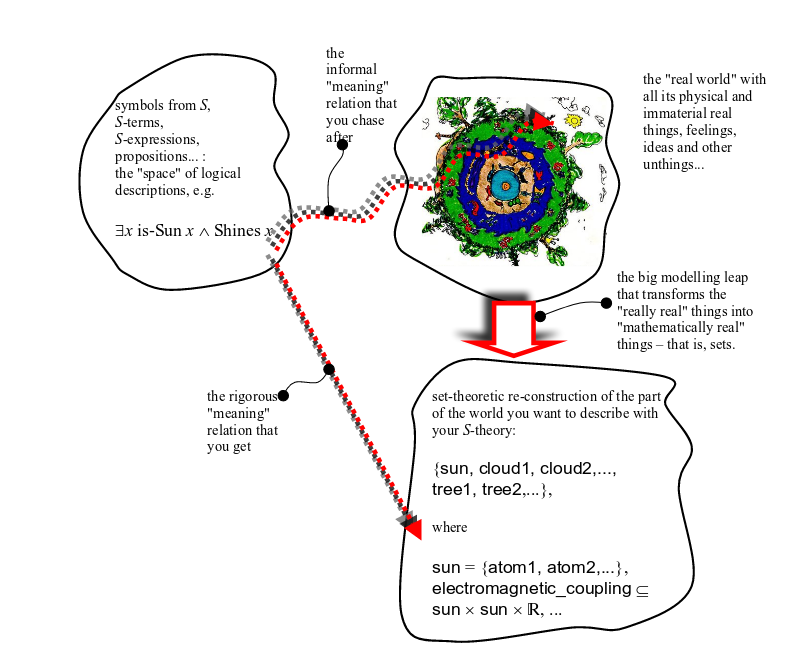
\includegraphics[width=6cm]{./triangulo} &
        \begin{itemize}
            \item{Dado un conjunto de reglas $\phi$ de un sistema}
            \item{Supongamos que $\psi$ expresa una utilizaci\'on indevida del sistema.}
            \item{Si $\phi\ \models\ \psi$, entonces nos pueden hakear.}
        \end{itemize}
    \end{tabular}
\end{frame}

\begin{frame}
    \frametitle{Seguridad: ¿Que puede salir mal?}
    {\bf ¡Muchas cosas!}, entre ellas:
    \begin{itemize}
        \item{Los datos se modifican de forma indevida.}
        \item{Un usuario obtiene acesso a datos que no puede ver.}
        \item{Un usuario escala sus privilegios en un sistema.}
        \item{Un usuario falsifica un documento.}
    \end{itemize}
    En resumen, a pesar que la criptografia y otros mecanismos son robustos,
    es muy dificil utilizarlas correctamente.
\end{frame}

\begin{frame}
    \frametitle{Seguridad: Injecci\'on de SQL y Ataques de XSS}
    \begin{itemize}
        \item{Un sitio web, app u otros solicita informaci\'on al usuario (ie. una busqueda).}
        \item{Esta informaci\'on luego se almacena en la base de datos.}
        \item{El sistema genera una solicitud a la base de datos con los datos ingresados
        \emph{sin hacer ning\'una validaci\'on}}
        \item{Los datos contienen codigo, ya sea SQL o Javascript.}
        \item{Sucede alguno de:
            \begin{itemize}
                \item{El codigo SQL solicita datos de la base de datos.}
                \item{El codigo SQL hace cambios en la base de datos.}
                \item{El codigo Javascript luego se presenta y ejecuta en paginas de otros ususarios.}
            \end{itemize}
        }
    \end{itemize}
\end{frame}

\begin{frame}
    \frametitle{Seguridad: Errores}
    {\bf Errores:}
    \begin{itemize}
        \item{{\bf Error \#1:} Confiar en los datos del usuario}
        \item{{\bf Error \#2:} No almacenar los datos privados de forma segura}
        \item{{\bf Error \#3:} Separaci\'on inapropiada de datos y codigo}
    \end{itemize}
    {\bf Observaciones:}
    \begin{itemize}
        \item{Este error fue muy comun en PHP. No por que PHP
        fuera inseguro como tal, sino que permitia que personas
        con poco conocimiento levantaran sitios web.}
        \item{La mayoria de los \emph{Web Frameworks} y \emph{ORMs}
        modernos automaticamente protegen la base de datos de estos
        errores asi que m\'as vale utilizar alguno.}
    \end{itemize}
\end{frame}

\begin{frame}
    \frametitle{Seguridad: Buffer Overflows}
    \begin{itemize}
        \item{Un sistema obtiene datos (generalmente un string)
        de un lugar externo al sistema.}
        \item{El sistema no valida la longitud ni contenido del
        string de forma adecuada.}
        \item{El sistema copia el string a un \emph{buffer} en
        la memoria, y no revisa el tama\~no del buffer.}
        \item{Por lo general se utiliza una funcion como
        \texttt{strcpy}, la cual no valida si el buffer tiene la
        capacidad necesaria.}
        \item{Al exceder la capacidad del buffer, parte del contenido
        del string se copia a la memoria del programa. Este contenido
        por lo general tiene codigo ejecutable.}
        \item{El comportamiento del programa cambia debido a que
        su memoria ahora tiene codigo introducido del exterior.}
    \end{itemize}
\end{frame}

\begin{frame}
    \frametitle{Seguridad: Errores}

    \begin{itemize}
        \item{{\bf Error \#1:} Confiar en datos externos al sistema}
        \item{{\bf Error \#2:} Separaci\'on incorrecta de datos y codigo}
        \item{{\bf Error \#3:} El sistema se ejecuta con privilegios elevados.}
    \end{itemize}
    {\bf Observaciones:}
    \begin{itemize}
        \item{Estas vulnerabilidades por lo general solo se dan en lenguajes
        de bajo nivel como C y C++.}
        \item{Muchos sistemas operativos y procesadores tienen mecanismos que
        permiten proteger la memoria contra modificaciones indebidas.}
        \item{¿Que patrones se repiten?}
    \end{itemize}
\end{frame}

\begin{frame}
    \frametitle{Referencias}
    \bibliography{../../Referencias/referencias}
    \bibliographystyle{plain}
\end{frame}

\end{document}